\documentclass[a4paper]{article}
\usepackage[UTF8]{ctex}
\usepackage{geometry}
\usepackage{graphicx}
\usepackage{url}
\usepackage{multirow}
\usepackage{array}
\usepackage{booktabs}
\usepackage{url}
\usepackage{enumitem}
\usepackage{graphicx}
\usepackage{float}
\usepackage{amssymb}
\usepackage{amsmath}
\usepackage{subfig}
\usepackage{longtable}
\usepackage{pifont}
\usepackage{color}

\allowdisplaybreaks

\geometry{a4paper, scale=0.78}

% \begin{figure}[H]
%     \centering
%     \includegraphics[width=.55\textwidth]{E.png}
%     \caption{矩阵与列向量的乘法}
%     
% \end{figure}

% \left\{
% \begin{array}{ll}
%       x+2x+z=2 & \\
%       3x+8y+z=12 & \\
%       4y+z=2
% \end{array}
% \right.

% \begin{enumerate}[itemindent = 1em, itemsep = 0.4pt, parsep=0.5pt, topsep = 0.5pt]

% \end{enumerate}

%\stackrel{a}{\longrightarrow}

\title{Probability Graph 10 Moral Graph \& Factor Graph}
\author{Chen Gong}
\date{11 December 2019}

\begin{document}
\maketitle
在这一小节中,我们将要介绍两种特殊的概率结构,也就是Moral Graph和Factor Graph。

\section{Moral Graph}
首先我们需要知道,为什么要有Moral Graph的存在?Moral Graph存在的意义就是将有向图转化为无向图来研究。因为无向图比有向图更加的Generalize一些。在概率图中,我们可以分为贝叶斯网络(有向图)和马尔可夫网络(无向图)。

无向图可以表示为:
\begin{equation}
    p(x) = \frac{1}{z}\prod_{i=1}^k \phi_{c_i}(x_{c_i})
\end{equation}

有向图可以表示为:
\begin{equation}
    p(x) = \prod_{i=1}^pp(x_i|x_{pa(i)})
\end{equation}

其中,$\phi_{c_i}$代表的是最大团的意思。通过道德图,我们可以有效的将有向图转换为无向图。

我们看一下如图所示的链式网络:
\begin{figure}[H]
    \centering
    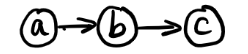
\includegraphics[width=.25\textwidth]{微信图片_20191211151651.png}
    \caption{链式有向图模型}
    
\end{figure}

其中,$p(a,b,c) = p(a)p(b|a)p(c|b)$。如果,把有向图转换成有向图是一件非常简单的事情,首先把所有的线条换成直线。由于在无向图中,我们考虑的是最大团,所以$p(a)p(b|a) = \varphi(a,b)$,$p(c|b) = \varphi(b,c)$。这个的转换是非常的简单了。

第二种,我们需要讨论的图也就是Tail to Tail的图,所下图所示:
\begin{figure}[H]
    \centering
    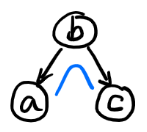
\includegraphics[width=.15\textwidth]{微信图片_20191211152752.png}
    \caption{Tail to Tail有向图模型}
    
\end{figure}

其中,$p(a,b,c) = p(a)p(b|a)p(c|a)$。还是按照一样的套路,首先把所有的有向箭头改成直线。那么我们就可以得到$p(a)p(b|a) = \phi(a,b)$,$p(c|a) = \phi(a,c)$。其中$\{a,c\}$和$\{b,c\}$是分别属于两个团。这个也比较的简单,但是Head to Head的转换就有点不一样了。

第三种,我们需要讨论的图是Head to Head的模型,如下图所示:
\begin{figure}[H]
    \centering
    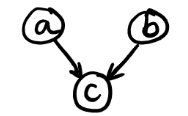
\includegraphics[width=.2\textwidth]{微信图片_20191211153908.png}
    \caption{Head to Head有向图模型}
    
\end{figure}

同样我们使用一样的分析思路来看这个问题,$p(a,b,c) = p(a)p(b)p(c|a,b)$。我们进行拆解的话,只能令$p(a)p(b)p(c|a,b) = \varphi(a,b,c)$,不然再也找不到其他的拆解方法。但是,如果简单的将模型中所有的有向箭头改成直线得到的并不是一个团。因为``团"的概念的要求,团里面的元素都要求是两两相互连接的。所以,我们需要进行改进,将Head to Head的无向图形式改进为:
\begin{figure}[H]
    \centering
    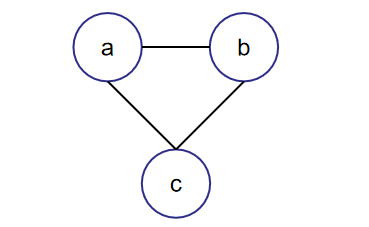
\includegraphics[width=.3\textwidth]{微信图片_20191211155130.png}
    \caption{Head to Head无向图模型}
    
\end{figure}

那么,将Head to Head的有向图转换为无向图的过程可以被我们描述为:

对于$\forall x_i \in G$,将$parent(x_i)$的两个父亲节点连接,然后将$G$中所有的有向边替换成无向边。下面我们举一个例子:
\begin{figure}[H]
    \centering
    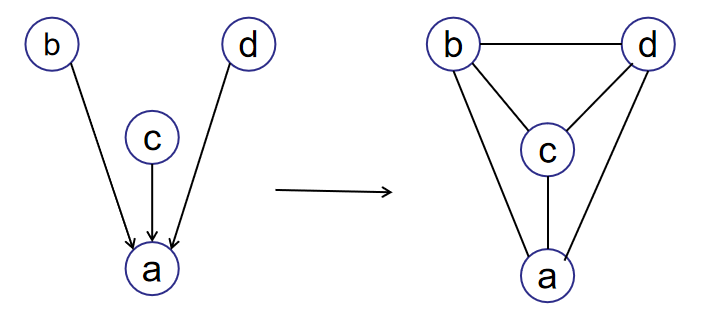
\includegraphics[width=.5\textwidth]{微信图片_20191211160601.png}
    \caption{Head to Head有向图模型转无向图模型举例}
    
\end{figure}

而我们将有向图转换成无向图之后,有什么好处吗?也就是在判断条件独立性的时候,有时图形非常复杂的时候。我们在有向图中很难看出来,而在无向图中却可以很简单的得到我们想要的结果。也就是$Sep(A,B|C) \Longleftrightarrow D-Sep(A,B|C)$。

\section{Factor Graph}
在上一小节中,我们介绍了道德图(Moral Graph),它的主要作用是将有向图转换为无向图。我们考虑的都是树结构,但是在Head to Head结构中,会引入环的结构。但是,在我们的Belief Propagation (BP)算法中,只能对树进行分解。所以,这里我们就引入了因子图。因子图主要发挥两个作用:1. 去环,也就是消除无向图中的环结构;2. 使算法变得更加的简洁,简化计算。

如图二表达的那样,他的有向图和无向图的联合概率可以分别表达为:
\begin{equation}
    p(a,b,c) = p(a)p(b|a)p(c|a) \qquad p(a,b,c) = \frac{1}{Z}\phi(a,b)\phi(a,c)
\end{equation}

那什么是因子图分解呢?公式表达可以被我们表示为:
\begin{equation}
    p(x) = \prod_{S}p(x_S)
\end{equation}

其中,$S$是图的节点子集,$X_S$为对应的$X$的子集,也就是$X$的随机变量的子集。那么对于一个如图4所示的有环无向图,我们怎么进行因子图分解呢?

首先进行第一种分解,如下图所示:
\begin{figure}[H]
    \centering
    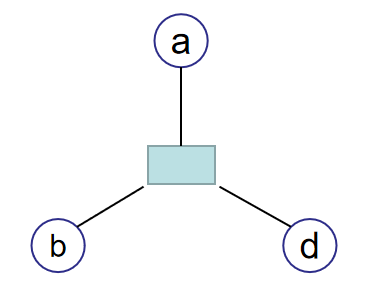
\includegraphics[width=.35\textwidth]{微信图片_20191212093305.png}
    \caption{Head to Head无向图中心节点因子图分解}
    
\end{figure}

这时可以被我们描述为,$f = f(a,b,c)$。或者我们也可以进行更细的分解。如下图所示:
\begin{figure}[H]
    \centering
    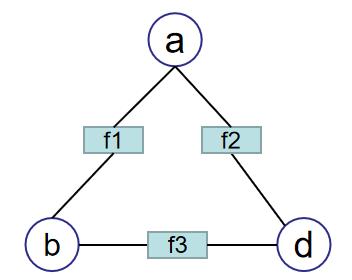
\includegraphics[width=.35\textwidth]{微信图片_20191212094218.png}
    \caption{Head to Head无向图三节点因子图分解}
    
\end{figure}


这个分解的结果可以被我们表示为:
\begin{equation}
    p(x) = f_1(a,b)f_2(a,c)f_3(b,c)
\end{equation}

不仅是可以在两个节点之间插入关系,同时也可以对于单个节点引入函数。
\begin{figure}[H]
    \centering
    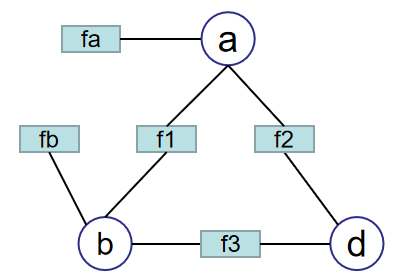
\includegraphics[width=.35\textwidth]{微信图片_20191212094923.png}
    \caption{Head to Head无向图三节点和独立节点因子图分解}
    
\end{figure}

那么这个分解结果可以被我们表示为:
\begin{equation}
    p(x) = f_1(a,b)f_2(a,c)f_3(b,c)f_a(a)f_b(b)
\end{equation}

实际上,就可以看成是对因式分解的进一步分解。这样我们就可以成功的消除环结构。如下图所示:
\begin{figure}[H]
    \centering
    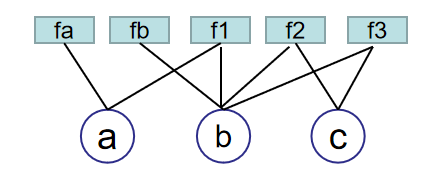
\includegraphics[width=.35\textwidth]{微信图片_20191212100021.png}
    \caption{Head to Head无向图三节点和独立节点因子图分解}
    
\end{figure}

所以,大家仔细一想就知道了因子图存在的意义了,它可以有效的消除环结构,通过一个重构的方式,重建出树的结构。这样可以有效的帮助我们使用Belief Propagation中的变量消除法等方法。

















\end{document}
